\subsection{Starky for ZKVM}\label{section: starky-zkvm}

At present, a zero-knowledge proof system consists of modules such as arithmetic, constraint system and polynomial commitment scheme. Ola's proof system is based on Starky, a complementary proof system developed by Polygon Zero. Starky uses the same finite field and hash functions as Plonky2 but without the computation-heavy arithmetizations. And so at the transaction level, Starky generates proofs in parallel. The arithmetic and constraint system in Starky is implemented using AIR. That is, the calculation process of the program is represented by several Stark tables, and there are constraint relationships between the rows and columns of tables, and also constraint relationships between different tables. The polynomial commitment scheme in Starky is FRI, a protocol that establishes that a committed polynomial has a bounded degree.

On the basis of Starky, we further optimized the performance and reduced the time to generate proofs by half.

\subsubsection{Field}\label{section: starky-field}

\noindent The difficulties of ZK-STARKs and ZK-SNARKs in dealing with integer operation are:

\begin{enumerate}
    \item All values are represented as finite field elements with large bit-width.
    \item It's expensive to convert finite field operations to 32-bit or 64-bit integer operations.
\end{enumerate}

\noindent Starky uses a small field called Goldilocks to perform field operations. Goldilocks field is a prime field of order $p = 2^{64} - 2^{32} + 1$. Goldilocks has the following properties:

\begin{enumerate}
    \item Each u32 operation requires only one VM cycle using the Goldilocks field.
    \item Field elements are within 64-bit, making operations on Goldilocks field fast on modern CPUs.
    \item There is no overflow problem in the modular multiplication operation of two 32-bit integers.
    \item It's very efficient to check whether 4 16-bit values can construct a valid field element.
\end{enumerate}

According to the test, a single multiplication operation on the Goldilocks field takes only 2\textasciitilde3 cycles on modern CPUs. In addition, the delay of multiplication is also lower and resource utilization is higher than other fields such as alt-bn128 and bn254.
\subsubsection{Generation of Stark Tables}\label{section: starky-geneartion-tables}

The program in Ola will generate multiple original STARK tables after execution. There are currently five tables of CPU, Memory, Bitwise, RangeCheck and CMP, and new tables may be added later.

Different tables define a different number of columns for storing data such as limbs, lookups, etc. The values of some columns are determined when the program is executed, and the values of the remaining columns need to be calculated using the program execution results. When the cells of all Stark tables have values, we get the complete Stark tables, and then we can use Fast Fourier transform to interpolate each column in each Stark table into a polynomial.The operation process for each table is as follows:
\subsubsection{Starky Proof Generation}\label{section: starky-generate-proof}

Once we have the polynomial array and public input for each STARK table as described in \figref{section: starky-generation-tables}, we can start the proving process. Each STARK table in Starky must generate a ZK-STARK proof separately. The proof process for each table is as follows:

\begin{enumerate}
    \item Compute Polynomials and Commitments.
        \begin{enumerate}
            \item Generate a Merkle commitment from polynomials of STARK table columns;
            \item Divide the instance of the permutation argument into multiple batches, each batch generates a polynomial $Z(X)$;
            \item Calculate $Z(X)$ polynomials for cross table lookups;
            \item Generate a Merkle commitment from all $Z(X)$ polynomials above.
        \end{enumerate}
    \item Using trace polynomials and $Z(X)$ to generate quotient polynomials:
        \[ \mathrm{quotient}(X) = \frac{\sum C(X) + (P\_Z(gX)\prod rhs - P\_Z(X)\prod lhs) + (CTL\_Z(gX) - CTL\_Z(X) \mathrm{selector}(gX))}{X^n - 1} \]
    \item Divide the quotient polynomials into small polynomials, the degrees of which are \verb|quotient_degree_factor|;
    \item Generate a Merkle commitment from quotient polynomials;
    \item Calculate the three points of the challenge $\zeta$, $g \cdot \zeta$ and the last point $ g^{n-1} $ in the group $H$;
    \item Open the challenge points on the polynomial, respectively, and get openings;
        \begin{enumerate}
        \item Point $\zeta$ is opened on
            \begin{itemize}
                \item Trace polynomials
                \item Permutation and cross table lookups polynomials
                \item Quotient polynomials
            \end{itemize}
        \item Point $g \cdot \zeta$ is opened on
            \begin{itemize}
                \item Trace polynomials
                \item Permutation and cross table lookups polynomials
            \end{itemize}
        \item Point $ g^{n-1} $ is opened only on
            \begin{itemize}
                \item Cross table lookups polynomials
            \end{itemize}
        \end{enumerate}
    \item Generate the final polynomial;
        \begin{enumerate}
            \item Compress the polynomial opened at each point into one polynomial $$ F_i(X) = \sum_{j} \alpha^j \cdot f_{ij}, i \in [3] $$
            \item Calculate the above $ F_i(X) $ quotient, where $ z \in \{ \zeta, g \cdot \zeta, g^{n-1} \} $ $$ Q_i(X) = \frac{F_i(X) - F_i(z)}{X - z} $$
            \item Compress all the points to $ Q_i(X) $ get the polynomial of the final FRI $$ \mathrm{Final}(X) = \sum_{k=0}^3 \alpha^k Q_i(X) $$
        \end{enumerate}
    \item Generate a FRI proof for the final polynomial fri\_proof;
    \item Finally got the proof of a single stark, proof consists of
        \begin{itemize}
            \item trace\_cap
            \item permutation\_ctl\_zs\_cap
            \item quotient\_polys\_cap
            \item openings
            \item fri\_proof
        \end{itemize}
    \item The STARK proofs and public input of all STARK tables are converted into a final proof of the program, called a Starky proof.
\end{enumerate}

\noindent There are now a total of 3 Merkle commitments

\begin{enumerate}
    \item A Merkle commitment of trace polynomials;
    \item A Merkle commitment of permutation\_ctl\_zs polynomials;
    \item A Merkle commitment of quotient polynomials.
\end{enumerate}

\noindent The order of a quotient polynomial is determined by the related constraints and trace degree: $$\mathrm{quotient\_degree\_factor} \cdot \mathrm{degree}$$ The last point $g^{n-1}$ is for cross table lookup checking. That is, the product of the last point value of multiple looking tables is equal to the last point value of the looked table.

\subsubsection{Starky Proof Verification}\label{section: starky-verify-proof}

Proving that an Ola program executes correctly requires verifying the starky proof generated in \ref{section: starky-generate-proof}. Verification mainly includes that each STARK proof is valid and that the cross table constraints between different STARK tables are correct. The process is as follows:

\begin{enumerate}
    \item Get all challenges for generating STARK proofs
    \item Get the number of Z polynomials  in permutation arguments
    \item Generate the data required to verify the Z polynomials of the cross table lookups
        \begin{enumerate}
            \item The values of Z polynomials at $\zeta$ and $g \cdot \zeta$ at each table generated
            \item Generate the required $\beta, \gamma$ used in generation of Z polynomials
            \item Columns and selectors used for cross table lookups in each STARK table
        \end{enumerate}
    \item Verify each stark proof individually
        \begin{enumerate}
            \item Check the number of polynomials and cap\_height of the stark proof are valid
            \item Get the value of 3 points ($\zeta$, $g \cdot \zeta$ and $g^{n-1}$) opened on column polynomials
            \item Calculate the values of constraints, permutation arguments, and cross table lookup polynomials at the above three points
            \item Check $quotient(\zeta) \cdot Z\_H(\zeta) = vanishing(\zeta)$
            \item Check FRI proof is valid
        \end{enumerate}
\end{enumerate}

\subsubsection{FRI}\label{section: starky-fri}

\begin{figure}[!htp]
    \centering
    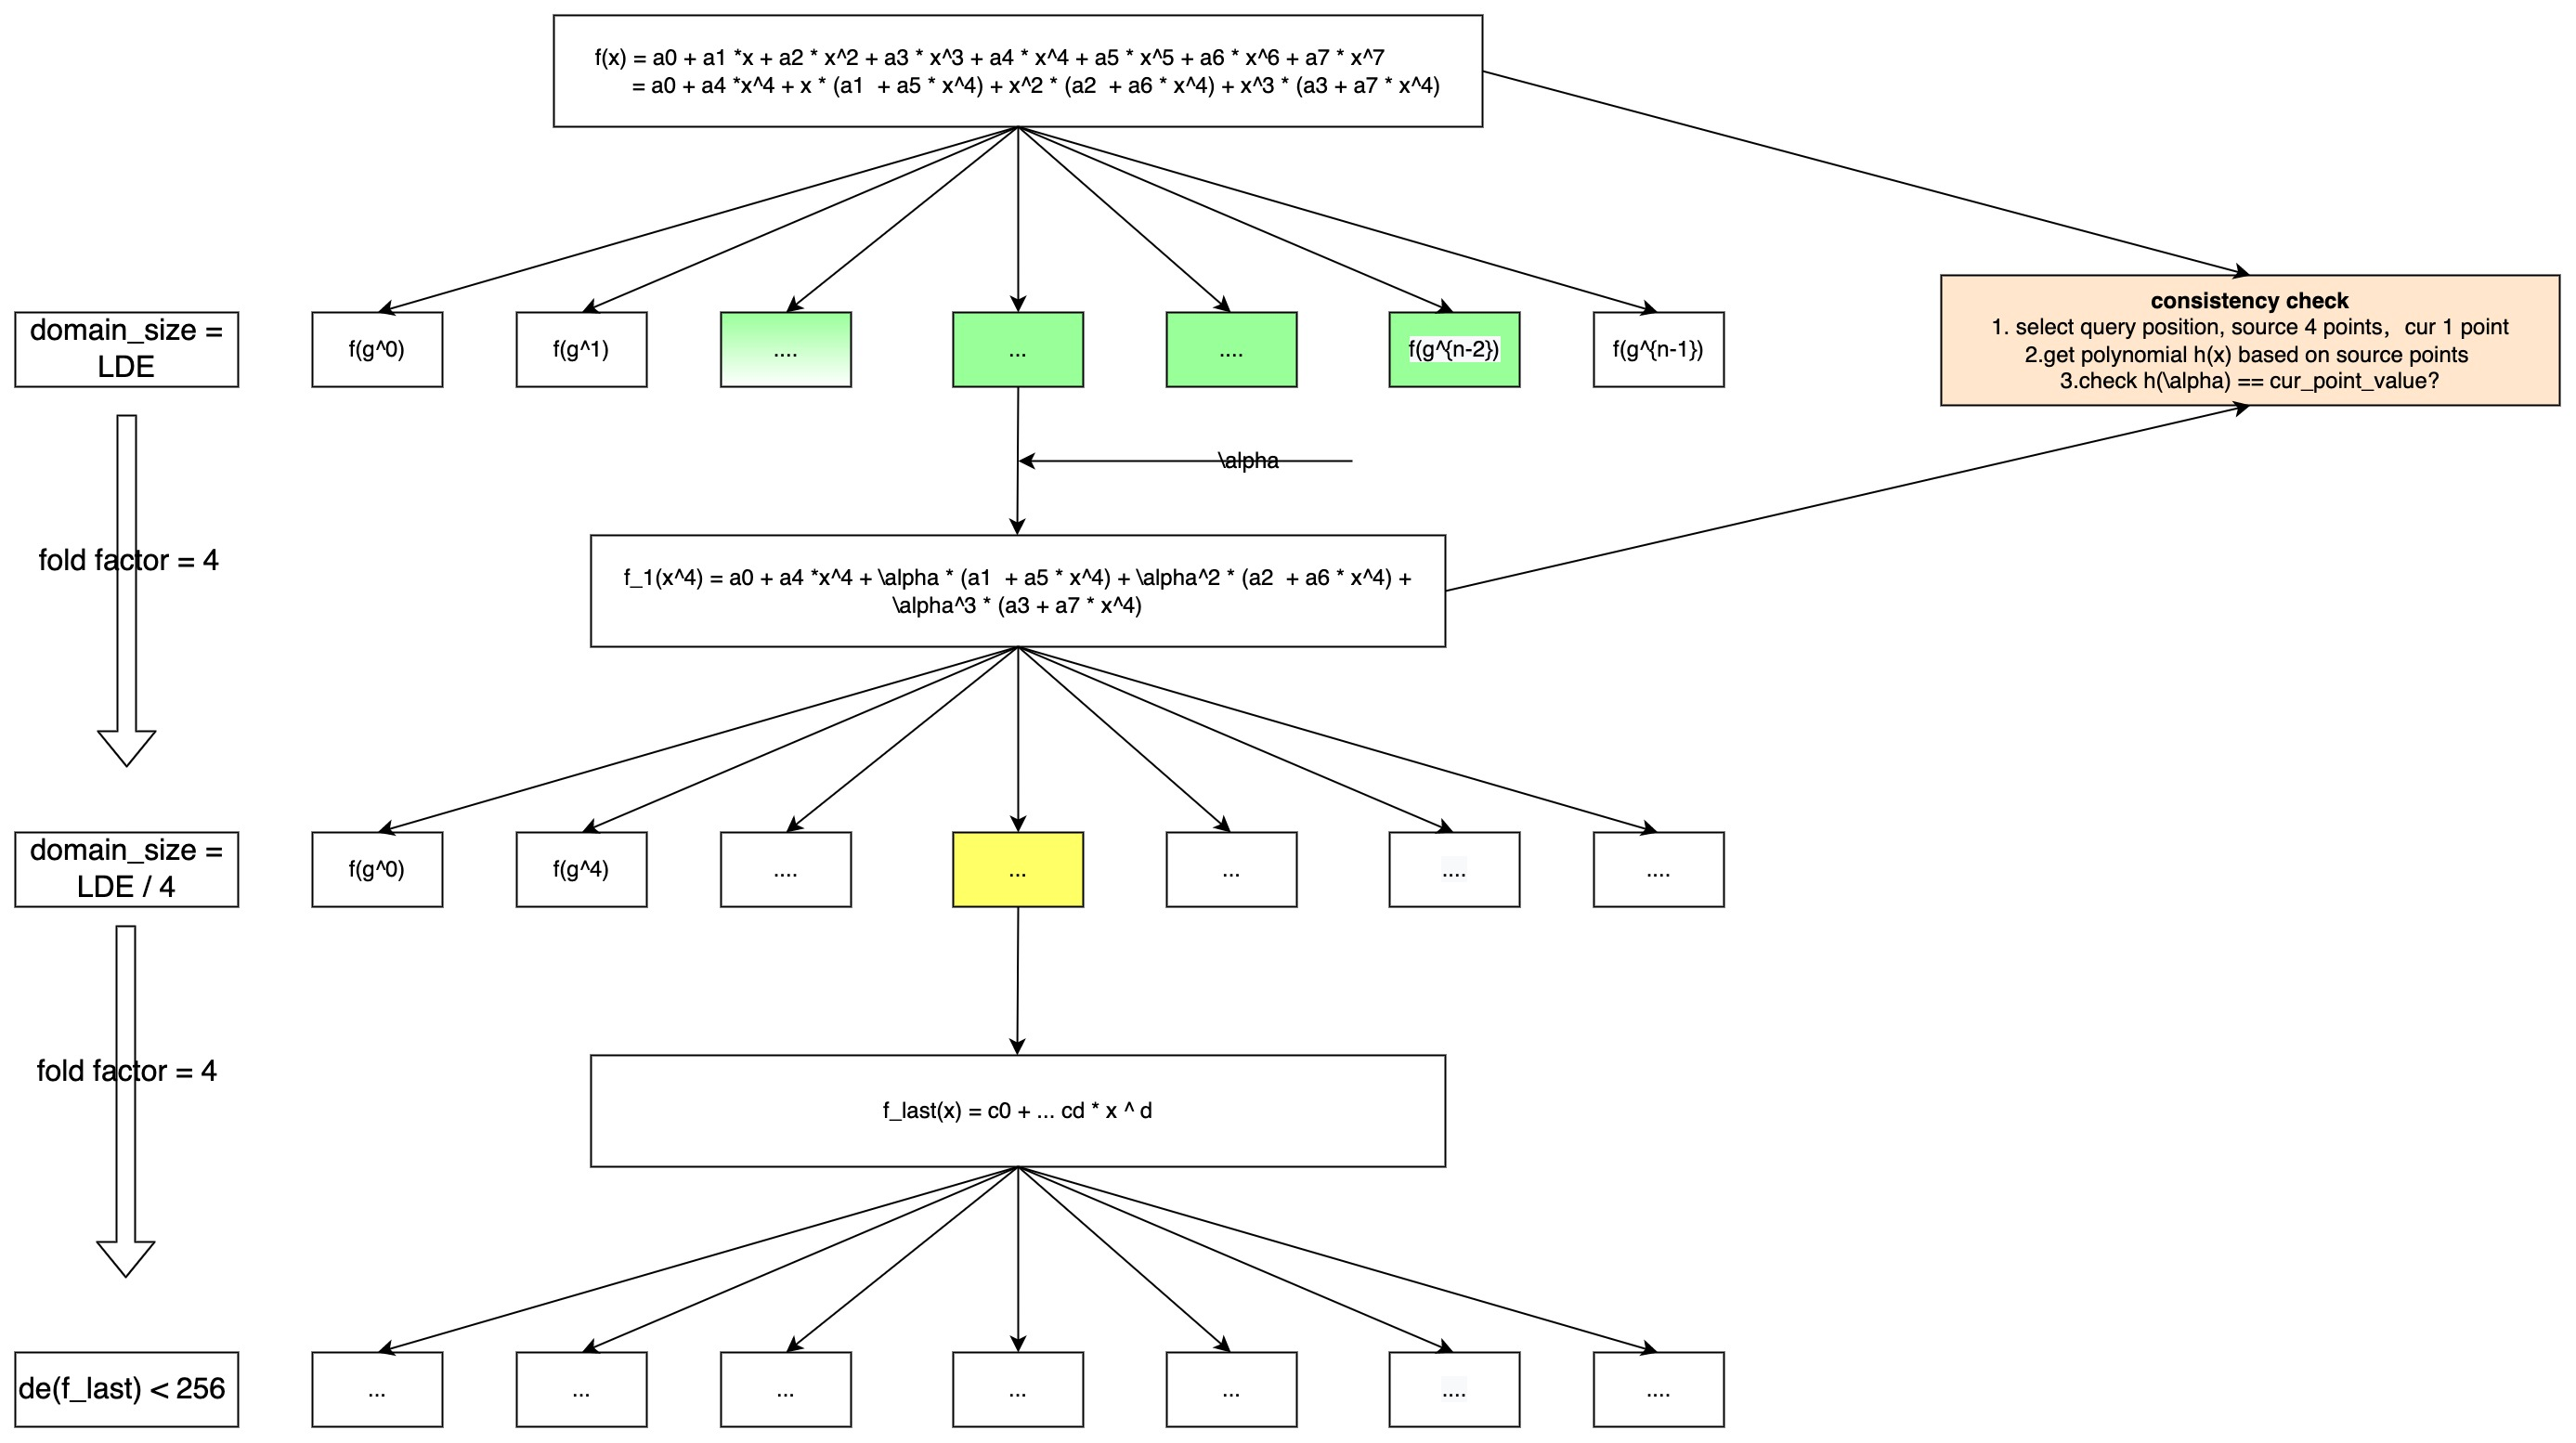
\includegraphics[width=0.8\textwidth]{fri.jpg}
    \caption{FRI protocol}
    \label{fig: FRI}
\end{figure}

FRI is a protocol that proves a committed polynomial having a bounded degree. Ola uses Deep-FRI for its polynomial commitment scheme. Figure \ref{fig: FRI} simply expresses the calculation process of FRI, anyone can read DEEP-FRI \cite{cryptoeprint:2019/336} for more details.
\subsubsection{Benchmark}\label{section: starky-benchmark}

Many optimizations have not yet been applied, and we expect to see more performance improvements as we devote more time to optimization. The benchmarks below should only be used as a rough guide to expected future performance.

In the benchmarks below, the VM executes the same Fibonacci calculator program for $2^{20}$ cycles at 100-bit target security level on an advanced 64-core CPU.

\begin{table}[!ht]
    \centering
    \begin{tabular}{|r|r|r|r|r|}
        \hline
        VM cycles & Execution time & Proving time & RAM consumption & Proof size \\
        \hline
        $2^{18}$ & 81.115 ms & 2.932 s & 5.6 GB & 175 KB \\
        \hline
        $2^{19}$ & 159.80 ms & 6.143 s & 11.1 GB & 181 KB \\
        \hline
        $2^{20}$ & 318.08 ms &12.688 s & 23.2 GB & 187 KB \\
        \hline
        $2^{21}$ & 627.38 ms & 29.923 s & 45.3 GB & 195 KB \\
        \hline
        $2^{22}$ & 1240.4 ms & 61.834 s & 86.6 GB & 208 KB \\
        \hline
        $2^{23}$ & 2453.8 ms & 128.62 s & 176 GB & 216 KB \\
        \hline
    \end{tabular}
\end{table}

